\chapter{Off-policy methods with approximation}

\section{Summary}

In the tabular case on-policy methods translate very easily to off-policy methods. This is not the case with the semi-gradient methods, the off-policy methods need \textbf{special care as converge is much harder to reach}.

The challenge of off-policy methods is split into 2 parts:
\begin{enumerate}
	\item update target
	\item change update distribution
\end{enumerate}

Some terminology used in this chapter:
\begin{itemize}
	\item $b$: behavior policy
	\item $\pi$: target policy
	\item $\hat{v} \approx v_{\pi}$
	\item $\hat{q} \approx q_{\pi}$
\end{itemize}

\subsection{Semi-Gradient methods}
Just as with the tabular algorithms we define the per-step importance sampling ratio as equation~\ref{eq:per-step importance sampling ratio}. The TD(0) algorithm then becomes equation~\ref{eq:semi-gradient TD(0) off-policy state-value update} and expected SARSA becomes~\ref{eq:semi-gradient expected sarsa off-policy action-value update}. 

\begin{equation}
\rho_t = \rho_{t:t} = \frac{\pi(A_t|S_t)}{b(A_t|S_t)}
\label{eq:per-step importance sampling ratio}
\end{equation}

\begin{equation}
\begin{split}
w_{t+1} & = w_t + \alpha \rho_t \delta_t \nabla \hat{v}(S_t, w_t) \\
\delta_t & = R_{t+1} + \gamma \hat{v}(S_{t+1}, w_t) - \hat{v}(S_t, w_t) \\
\delta_t & = R_{t+1} - \bar{R}_t + \hat{v}(S_{t+1}, w_t) - \hat{v}(S_t, w_t) \\
\end{split}
\label{eq:semi-gradient TD(0) off-policy state-value update}
\end{equation}

Expected SARSA without approximation doesn't need the importance sampling as it check's all future actions. The \textbf{approximation} however should take into account the \textbf{contribution of a certain state-action}. This is not handled yet is this formulation.

\begin{equation}
\begin{split}
w_{t+1} & = w_t + \alpha \delta_t \rho_t \nabla \hat{q}(S_t, A_t, w_t) \\
\delta_t & = R_{t+1} + \gamma \sum_{a} p(a|S_{t+1})\hat{q}(S_{t+1}, a, w_t) - \hat{q}(S_t, w_t) \\
\delta_t & = R_{t+1} + \bar{R}_t + \gamma \sum_{a} p(a|S_{t+1})\hat{q}(S_{t+1}, a, w_t)  - \hat{v}(S_t, w_t) 
\end{split}
\label{eq:semi-gradient expected sarsa off-policy action-value update}
\end{equation}

%The n-step sarsa can be generalized in the same way as illustrated by equation~\ref{eq:n-step SARSA semi-gradient}.

\begin{equation}
\begin{split}
w_{t+n} & = w_{t+n-1} + \alpha \rho_{t+1} ... \rho_{t+n-1}\Big[ G_{t:t+n}-\hat{q}(S_t, A_t, w_{t+n-1}) \Big] \nabla \hat{q}(S_t, A_t, w_{t+n-1})\\
G_{t:t+n} & = R_{t+1} + ... \gamma^{n-1}R_{t+n} + \gamma^n \hat{q}(S_{t+n}, A_{t+n}, w_{t+n-1}) \\
G_{t:t+n} & = R_{t+1} - \bar{R}_{t} + ... R_{t+n} - \bar{R}_{t+n-1} +  \hat{q}(S_{t+n}, A_{t+n}, w_{t+n-1}) \\
\end{split}
\label{eq:n-step SARSA semi-gradient}
\end{equation}

The tree backup algorithm doesn't need importance sampling and can be converted into a offline version (equation~\ref{eq:semi-gradient n-step tree backup algorithm offline}).

\begin{equation}
\begin{split}
w_{t+n} & = w_{t+n} + \alpha \Big[ G_{t:t+n} - \hat{q}(S_t, A_t, w_{t+n-1}) \nabla \hat{q}(S_t, A_t, w_{t+n-1}) \Big] \\
G_{t:t+n} & = \hat{q}(S_t, A_t, w_{t-1}) + \sum_{k=t}^{t+n-1} \delta_k \prod_{i=t+1}^{k}\gamma\pi(A_i|S_i) \\
\delta_t & = R_{t+1} + \gamma \sum_{a} p(a|S_{t+1})\hat{q}(S_{t+1}, a, w_t) - \hat{q}(S_t, w_t) \\
\delta_t & = R_{t+1} + \bar{R}_t + \gamma \sum_{a} p(a|S_{t+1})\hat{q}(S_{t+1}, a, w_t)  - \hat{v}(S_t, w_t) \\
\end{split}
\label{eq:semi-gradient n-step tree backup algorithm offline}
\end{equation}

\subsection{Off-policy divergence}
Bairds counter example illustrated in figure~\ref{fig:bairds counter example} will diverge on some off-policy methods. Exercise 11.3 uses Q-learning, and the weights diverge. It does converge with on-policy methods, so off-policy methods need a bit of special care.

\begin{itemize}
	\item $b$: dashed lines p=6/7, solid lines p=1/7
	\item $\pi$: always solid lines
	\item reward=0 on all transitions
	\item discount rate is $\gamma=0.99$
\end{itemize}

\begin{figure}[H]
	\centering
	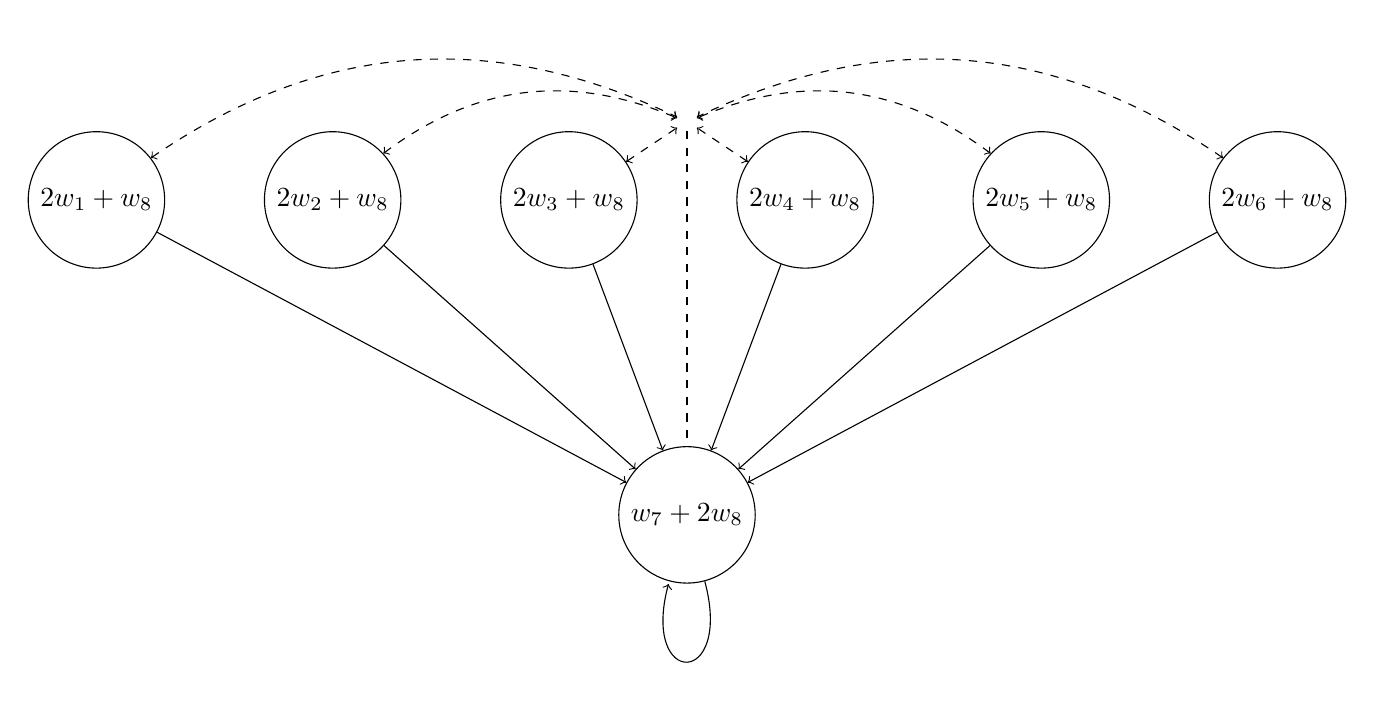
\begin{tikzpicture}
	
	\node[circle, draw] at (0, 0) (a) {$2w_1 + w_8$};
	\node[circle, draw] at (3, 0) (b) {$2w_2 + w_8$};
	\node[circle, draw] at (6, 0) (c) {$2w_3 + w_8$};
	\node[circle, draw] at (9, 0) (d) {$2w_4 + w_8$};
	\node[circle, draw] at (12, 0) (e) {$2w_5 + w_8$};
	\node[circle, draw] at (15, 0) (f) {$2w_6 + w_8$};
	
	\node[circle, draw] at (7.5, -4) (g) {$w_7 + 2w_8$};
	\node[] at (7.5, 1) (gup) {};
	
	\draw[] [->, auto] (a) to node {} (g);
	\draw[] [->, auto] (b) to node {} (g);
	\draw[] [->, auto] (c) to node {} (g);
	\draw[] [->, auto] (d) to node {} (g);
	\draw[] [->, auto] (e) to node {} (g);
	\draw[] [->, auto] (f) to node {} (g);
	
	\draw[dashed] [<->, auto, bend left] (a) to node {} (gup);
	\draw[dashed] [<->, auto, bend left] (b) to node {} (gup);
	\draw[dashed] [<->, auto] (c) to node {} (gup);
	\draw[dashed] [<->, auto] (d) to node {} (gup);
	\draw[dashed] [<->, auto, bend right] (e) to node {} (gup);
	\draw[dashed] [<->, auto, bend right] (f) to node {} (gup);
	
	\draw[dashed] [-, auto] (gup) to node {} (g);
	
	\path (g) edge [loop below] node {} (g);
	
	\end{tikzpicture}
	\caption{Bairds counter example}
	\label{fig:bairds counter example}
\end{figure}

Some approximation methods do not extrapolate from the observed targets, and so are always stable. These are called \textbf{averagers}, and include weighted regression and nearest neighbors. But not the more popular methods such as tile coding and artificial neural networks. (ANNs)

\subsection{The Deadly Triad}
The dangerous instability of off-policy methods occurs when combining 3 elements, these are called \textbf{The Deadly Triads}.

\begin{itemize}
	\item \textbf{Function approximation}: A way of generalizing from a state-space.
	\item \textbf{Bootstrapping}: Update targets using estimates, and not exclusively using actual rewards.
	\item \textbf{Off-Policy training}: Training on a distribution of transitions other than that produces by the target policy.
\end{itemize}

All tree elements are often required, function approximation is needed to generalize on large problems. Bootstrapping speeds up convergence, and lowers memory usage. For example Monte-Carlo methods use no bootstrapping but require you to put the entire trajectory in memory. (which might be very big) And finally off-policy learning is required to learn specific aspects of a process, just like humans do.

\subsection{Linear Value-function Geometry}
The distance between two value functions $||v_1 - v_2||^2_\mu$ is defined using the norm of equation~\ref{eq:value function norm}, it takes into account the importance of the states using $\mu(s)$.

\begin{equation}
||v||^2_\mu = \sum_{s\in S}\mu(s)v(s^2)
\label{eq:value function norm}
\end{equation}

\begin{equation}
\Pi v = v_w \text{ where } w=\argmin_{w\in \Re^d}|| v-v_w ||^2_\mu
\label{eq:projection operator closes approximated value function}
\end{equation}

In Monte-Carlo estimation the value function is approximated using the operator $\Pi$ defined in equation~\ref{eq:projection operator closes approximated value function}. It minimizes the squared distance between the exact $v_\pi$ and approximated $v_w$. The TD methods however find an other value function using the bellman operator (equation~\ref{eq:bellman operator}).

\begin{equation}
v_\pi(s) = \sum_a \pi(a|s) \sum_{s',r}p(s', r)[r+\gamma v_{\pi}(s')]
\label{eq:chapter11 bellman equation}
\end{equation}
The bellman equation (equation~\ref{eq:chapter11 bellman equation}) leads to the Bellman error equation (equation~\ref{eq:bellman error vector}). The bellman error is the expected value of the TD-error (per state notice $\bar{\delta}_w(s)$ is in function of $s$).
\begin{equation}
\begin{split}
\bar{\delta}_w(s) & = \Big( \sum_a \pi(a|s) \sum_{s', r} p(s', r | a, s)[r+\gamma v_w(s')] \Big) - v_w(s) \\
& = \EX\big[ R_{t+1} + \gamma v_w(S_{t+1}) - v_w(S_t) | S_t = s, A_t \sim \pi \big]\\
\end{split}
\label{eq:bellman error vector}
\end{equation}

The Mean Squared Bellman error $\overline{BE}$ of equation~\ref{eq: Mean Squared Bellman error} indicates the overall error in the value function.
\begin{equation}
\overline{\text{BE}}(w) = || \bar{\delta}_w ||^2_\mu
\label{eq: Mean Squared Bellman error}
\end{equation}
By applying the Bellman operator of equation~\ref{eq:bellman operator} to the value function repeatably $v_\pi = B_\pi v_\pi$ to the optimal approximated value function is obtained as the fixed point.
\begin{equation}
(B_\pi v)(s) = \sum_a \pi(a|s) \sum_{s', r} p(s', r | s, a)[r+\gamma v(s')]
\label{eq:bellman operator}
\end{equation}
For any approximated value function $v$, we define the \textbf{Mean Square Projected Bellman Error} as $\overline{PBE}$ (equation~\ref{eq:Mean Squared Projected Bellman Error}). With linear approximation there always exists a vector $w$ where $\overline{PBE}(w_{optimal})=0$. This however does not mean that the point $w_{optimal}$ is always stable under off-policy training.
\begin{equation}
\overline{PBE}(w) = || \Pi\bar{\delta}_w||^2_\mu
\label{eq:Mean Squared Projected Bellman Error}
\end{equation}

\fbox{
\begin{minipage}{11cm}
\begin{equation}
v_w = Xw
\end{equation}
The linear approximation $v=w^Tx_s$ defines a feature vector $x_s$ that expresses the relation between a state and the weights that leads to the value of the value function. These vectors are referred to as feature vectors. The matrix $X$ contains all the feature vectors in its rows, diagonal matrix $D$ contains the weights of the states $\mu(s)$.

\begin{equation}
X^+ = (X^TDX)^{-1}X^TD
\label{eq:pseudo inverse of weighted least square}
\end{equation}
Equation~\ref{eq:pseudo inverse of weighted least square} is the pseudo inverse of a weighted least square approximation of the value function using the feature vectors in $X$. The pseudo inverse find the weights that lead to the value function, and if these weights are multiplied by the feature vectors you get the linear value function. (every row of $X$ multiplied by $w$ results in a value per state).

\begin{equation}
\begin{split}
v_w &= \Pi v \\
 &= X(X^{+}v) \\
 &= Xw \\
\end{split}
\end{equation}
\end{minipage}	
}

\subsection{Gradient Descent in the Bellman error}
Until now only the \textbf{Monte-Carlo methods were true gradient descent methods}, and so they always converge robustly. A naive approach would be to use the \textbf{expected square of the TD error}(slightly different from bellman error) as an objective function as illustrated by equation~\ref{eq:mean squared TD error}. 
\begin{equation}
\delta_t = R_{t+1} + \gamma \hat{v}(S_{t+1}, W_t) - \hat{v}(S_t, W_t)
\end{equation}
\begin{equation}
\begin{split}
\overline{TDE} & = \sum_{s\in S} \mu(s) \EX[\delta_t^2 | S_t, A_t \sim \pi] \\
& = \sum_{s\in S} \mu(s) \EX[\rho_t \delta_t^2 | S_t, A_t \sim b] \\
& = \EX_b[\rho_t \delta^2_t] \text{   (if $\mu$ is the distribution encountered under b)}
\end{split}
\label{eq:mean squared TD error}
\end{equation}

The SGD per-step update becomes equation~\ref{eq:SGD per-step update mean squared TD error}. This is the same as the semi-gradient TD update except for the last term $\gamma \nabla\hat{v}(S_{t+1},w_t)$. This algorithm is referred to as \textbf{the naive residual-gradient algorithm}. It converges robustly, but not necessary to an optimal value function.
\begin{equation}
\begin{split}
w_{t+1} & = w_t - \frac{1}{2}\alpha \nabla(\rho_t \delta_t^2) \\
& = w_t - \alpha \rho^t \delta_t \nabla\delta_t \\
& = w_t + \alpha \rho_t\delta_t(\nabla \hat{v}(S_t, w_t) - \gamma \nabla \hat{v}(S_{t+1}, w_t)) 
\end{split}
\label{eq:SGD per-step update mean squared TD error}
\end{equation}

The minimization of $\overline{TDE}$ doesn't always accurately predict. A minimization of the \textbf{bellman error}(TD error in a particular state) however should result in a accurate prediction.

\begin{equation}
\nabla \delta_t = \gamma \nabla\hat{v}(S_{t+1}, W_t) - \nabla\hat{v}(S_t, W_t)
\label{eq:gradient TD error}
\end{equation}

\begin{equation}
\begin{split}
w_{t+1} & = w_t - \frac{1}{2} \alpha \nabla (\EX_{\pi}[{\delta_t^2}]) \\
& = w_t - \frac{1}{2}\alpha\nabla(\EX_b[\rho_t\delta_t]^2) \\
& = w_t - \alpha \EX_b[\rho_t\delta_t] \nabla\EX_b[\rho_t\delta_t] \\
& = w_t - \alpha \EX_b[\rho_t(R_{t+1} + \gamma \hat{v}(S_{t+1}, w) - \hat{v}(S_t, w))] \EX_b[\rho_t\nabla\delta_t] \\
& = w_t - \alpha \Big[\EX_b[\rho_t(R_{t+1} + \gamma \hat{v}(S_{t+1}, w)] - \hat{v}(S_t, w))\Big] \\ 
& \qquad \Big[ \EX_b[\rho_t (\gamma \nabla\hat{v}(S_{t+1}, W_t) )] - \nabla\hat{v}(S_t, W_t) \Big]\\
& = w_t + \alpha \Big[\EX_b[\rho_t(R_{t+1} + \gamma \hat{v}(S_{t+1}, w)] - \hat{v}(S_t, w))\Big] \\ 
& \qquad \Big[  \nabla\hat{v}(S_t, W_t) - \gamma\EX_b[\rho_t \nabla\hat{v}(S_{t+1}, W_t) ]\Big]\\
\end{split}
\end{equation}

\textbf{note:} $\rho_t$ stays inside the expected values, as its the importance sampling and depending on $\sim b$.

This algorithm is called \textbf{residual-gradient}, the two expected values need seperate sample's in order for the algorithm not to be biased. There are two way's to make this algorithm work:
\begin{enumerate}
	\item If the next state is deterministic, then 2 next samples will be the same, and the naive approach will work.
	\item If there is a simulator simply roll-back on $S_{t+1}$ and get a second sample.
\end{enumerate}
The residual-gradient algorithm is a true SGD algorithm and converges robustly with both linear and non-linear function approximation. In the linear case the solution is optimal and unique. 

However:
\begin{itemize}
	\item The residual-gradient algorithm is much slower then the semi-gradient
	\item If there is true function-approximation the minimum of $\overline{BE}$ is not the optimal value. (see drawing page 267 $\overline{BE}$ is not at same spot as $\Pi v_\pi$)
	\item "The bellman error is no learn-able" (next subsection)
\end{itemize}

\subsection{The Bellman Error is Not Learnable}
Typically the term "learnable" is used to define value's that can be learned in a polynomial amount of data.  It turns out that there are things that can't be "learned", no matter the amount of data. (example lower half of page 274).

So Some properties can be calculated using knowledge of the internal structure but can't be learned from the outside no matter how much data there is. The Bellman Error $\overline{BE}=||\delta_w||^2_\mu$ is such a property, as is the value error $\overline{VE}=||v_w - v_\pi||^2_\mu$, but the parameter $w$ that optimizes $\overline{VE}$ is observable.

\textbf{The mean square return error} defined in equation~\ref{eq:Mean Square Return Error} is the expectation under $\mu$. It is always observable, and it is equal to $\overline{VE}$ plus a variance term that does not depend on $w$. So the \textbf{optimum of $\overline{VE}$ for w must also be observable}.
\begin{equation}
\begin{split}
\overline{RE} & = \EX[(G_t - \hat{v}(S_t, w))^2] \\
& = \overline{VE}(w) + \EX[(G_t-v_{\pi}(S_t))^2] \\
\end{split}
\label{eq:Mean Square Return Error}
\end{equation}

In summary
\begin{itemize}
	\item $\overline{PBE}$ and $\overline{TDE}$ can be learned from the data. However there optimums differ from each other and $\overline{BE}$.
	\item $\overline{BE}$ is not at all learn-able, knowledge of the internal structure of the MDP is required to optimize $\overline{BE}$. The Residual gradient algorithm requires sampling from the same state twice. This obviously requires internal knowledge of the MDP.
\end{itemize}

\subsection{Gadient-TD Methods}
Equation~\ref{eq:regular least squares using pseudo inverse} is the regular least square, equation~\ref{eq:weighted least squares} contains the weighted least squares. Taking $W$ as a diagonal matrix with the weights. 
\begin{equation}
\begin{split}
A^+ & = (A^T A)^{-1}A^T \\
y & = A^+x
\end{split}
\label{eq:regular least squares using pseudo inverse}
\end{equation}
\begin{equation}
y = [(A^TWA)^{-1}X^TW]x
\label{eq:weighted least squares} 
\end{equation}

So assuming linear approximation(weighted least squares) $\Pi=X(X^TDX)^{-1}X^TD$ we can rewrite the objective function $\overline{PBE}$, using $\Pi^TD\Pi=DX(X^TDX)^{-1}X^TD$. $X$ is the matrix with the feature vectors of each state in its rows, D is a diagonal matrix with the state weights of $\mu(s)$. $\bar{\delta}_w$ is the bellman error of equation~\ref{eq:bellman error vector}.
\begin{equation}
\begin{split}
\overline{PBE}(w) & = ||\Pi\bar{\delta}_w||^2_\mu \\
& = (\Pi\bar{\delta}_w)^TD\Pi\bar{\delta}_w \\
& = \bar{\delta}^T_w\Pi^TD\Pi\bar{\delta}_w \\
& = \delta_w^TDX(X^TDX)^{-1}X^TD\bar{\delta}_w \\
& = (X^TD\bar{\delta}_w)^T(X^TDX)^{-1}(X^TD\bar{\delta}_w)
\end{split}
\end{equation}

The gradient with respect to $w$ becomes
\begin{equation}
\nabla\overline{PBE} = 2 \nabla [X^TD\bar{\delta}_w]^T (X^TDX)^{-1} (X^TD\bar{\delta}_w)
\end{equation}
Simplify the terms:
\begin{equation}
X^TD\bar{\delta}_w = \sum_s \mu(s)x(s)\bar{\delta}_w(s) = \EX[\rho_t\delta_tx_t]
\end{equation}
\begin{equation}
\begin{split}
\nabla \EX[\rho_t\delta_tx_t]^T & = \EX[\rho_t\nabla\delta_t^Tx_t^T] \\
& = \EX[\rho_t \nabla(R_{t+1} + \gamma w^Tx_{t+1} - w^Tx_t)^Tx_t^T] \\
& = \EX[\rho(\gamma x_{t+1} - x_t)x_t^T]
\end{split} 
\end{equation}
\begin{equation}
X^TDX = \sum_s \mu(s)x_sx_s^T = \EX[x_tx_t]
\end{equation}

Note that $x_t$ is the same as $x(s_t)$. Putting all the terms back together:
\begin{equation}
\nabla \overline{PBE}(s) = 2\EX[\rho_t(\gamma x_{t+1}-x_t)x^T_t]\EX[x_tx_t^T]^{-1}X[\rho_t\delta_tx_t]
\label{eq:PBE objective function rewritten with expectations}
\end{equation}
 
The 2th and 3th term of equation~\ref{eq:PBE objective function rewritten with expectations}, we will call $v$ can be estimated. Estimating $v$ is equivalent to approximating $\rho_t\delta_t$ from the features $X$ in a mean least-square sense. (notice the pseudo inverse in the formula). The SGD step to solve this is augmented with $\rho_t$ the sample ration and displayed in equation~\ref{eq:SGD on rho delta LMS}.
\begin{equation}
v\approx\EX[x_tx_t^T]^{-1}X[\rho_t\delta_tx_t]
\label{eq:PBE objective last 2 terms approximation}
\end{equation}
\begin{equation}
v_{t+1} = v_t + \beta \rho_t (\delta_t -v_t^Tx_t)x_t
\label{eq:SGD on rho delta LMS}
\end{equation}

The approximation of equation~\ref{eq:PBE objective last 2 terms approximation} is substituted in equation~\ref{eq:PBE objective function rewritten with expectations} resulting in equation~\ref{eq:GTD2}. This algorithm is called GTD2.

\begin{equation}
\begin{split}
w_{t+1} &= w_t - \frac{1}{2}\alpha\nabla\overline{PBE}(w_t) \\
&= w_t - \frac{1}{2}\alpha 2\EX[\rho_t(\gamma x_{t+1}-x_t)x^T_t]\EX[x_tx_t^T]^{-1}X[\rho_t\delta_tx_t] \\
&= w_t + \alpha\EX[\rho_t(x_t - \gamma x_{t+1})x^T_t]\EX[x_tx_t^T]^{-1}X[\rho_t\delta_tx_t] \\
&\approx w_t + \alpha \EX[\rho_t(x_t - \gamma x_{t+1})x^T_t] v_t \\
&\approx w_t + \alpha \rho_t (x_t - \gamma x_{t+1})x_t^Tv_t
\label{eq:PBE objective update step with approximation of last 2 terms}
\end{split}
\end{equation}

If more analytical steps are applied to equation~\ref{eq:PBE objective update step with approximation of last 2 terms} before approximating we get equation~\ref{eq:GTD0} with is called \textbf{TD(0) with gradient correction TDC} or alternatively the GTD0 algorithm.

\begin{equation}
\begin{split}
w_{t+1}&= w_t + \alpha\EX[\rho_t(x_t - \gamma x_{t+1})x^T_t]\EX[x_tx_t^T]^{-1}X[\rho_t\delta_tx_t] \\
&= w_t + \alpha(\EX[\rho_tx_tx^T] - \gamma\EX[\rho_t x_{t+1}x^T_t])\EX[x_tx_t^T]^{-1}X[\rho_t\delta_tx_t] \\
&= w_t + \alpha(\EX[x_tx^T] - \gamma\EX[\rho_t x_{t+1}x^T_t])\EX[x_tx_t^T]^{-1}X[\rho_t\delta_tx_t] \\
&= w_t + \alpha\Big(\EX[\rho_t\delta_tx_t] - \gamma\EX[\rho_t x_{t+1}x^T_t]\EX[x_tx_t^T]^{-1}X[\rho_t\delta_tx_t]\Big) \\
&\approx w_t + \alpha\Big(\EX[\rho_t\delta_tx_t] - \gamma\EX[\rho_t x_{t+1}x^T_t] v_t \Big) \\
&\approx w_t + \rho_t\alpha(\delta_tx_t - \gamma x_{t+1}x^T_t v_t )
\end{split}
\label{eq:GTD0}
\end{equation}

Both TDC and GTD3 learn 2 parameters, primary $w$ and secondary $v$. The primary learning process relies on the secondary to have learned at least some approximation. This asynchronous relation is called a cascade.

\subsection{Empathic-TD methods}
In off-policy learning actions/state-transitions are re-weighted according to their distribution. The states however are not re-weighted, if we were able to re-weight the states we would get as stable results on the off-policy as on-policy.

on page 282 it is rather unclear how the examples given and the TD-empathic algorithm relate to Pseudo termination.

\textbf{Pseudo termination} is termination that does not effect the sequence of state transitions, but does affect the learning process and the quantities being learned.

\begin{equation}
\begin{split}
\delta_t & = R_{t+1} + \gamma \hat{v}(S_{t+1}, w_t) - \hat{v}(S_t, w_t) \\
w_{t+1} & = w_t + \alpha M_t \rho_t \delta_t \nabla \hat{v}(S_t, w_t) \\
M_t & = \gamma \rho_{t-1} M_{t-1} + I_t
\end{split}
\label{eq:empathic-TD methods}
\end{equation}

\begin{itemize}
	\item $I_t$: interest, initialized arbitrary
	\item $M_t$: emphasis, initialized to $M_{t-1}=0$
\end{itemize}

\subsection{Reducing variance}
When using off-policy the behavior policy should not be too different from the target policy, as it might end up being rather absurd and we end up learning nothing. The behavior policy must must also not be too similar, as to actually learn new things.

Important sampling is useful to speedup the convergence. However it adds variance to the step size. Which might end up messing up the SGD, as it oversteps on a gradient. One solution to this is to use "adaptive step size algorithms". An other is to avoid to different behavior policy's, if the actions are not that different from the target policy. The variance on $\rho$ is small.

\section{Exercises}

\subsection{Exercise 11.1 page 259}
\textbf{Convert the equation of n-step off-policy TD to semi-gradient form. Give accompanying definitions of the return for both the episodic and continuing case.}

\begin{equation}
V_{t+n}(S_t) = V_{t+n-1}(S_t) + \alpha \rho_{t:t+n+1} \Big[ G_{t:t+n} - V_{t+n+1}(S_t) \Big]
\tag{equation 7.9 from the book page 148}
\end{equation}
Very similar to equation~\ref{eq:n-step SARSA semi-gradient}:
\begin{equation}
\begin{split}
w_{t+n} & = w_{t+n-1} + \alpha \rho_{t+1} ... \rho_{t+n-1}\Big[ G_{t:t+n}-\hat{v}(S_t, w_{t+n-1}) \Big] \nabla \hat{v}(S_t, w_{t+n-1}) \\
G_{t:t+n} & = R_{t+1} + ... \gamma^{n-1}R_{t+n} + \gamma^n \hat{v}(S_{t+n}, w_{t+n-1}) \\
G_{t:t+n} & = R_{t+1} - \bar{R}_{t} + ... R_{t+n} - \bar{R}_{t+n-1} +  \hat{v}(S_{t+n}, w_{t+n-1})
\end{split}
\end{equation}

\subsection{Exercise 11.2 page 259}
\textbf{Convert the equations of n-step $Q(\omega)$ to semi-gradient form. Give definitions that cover both the episodic and continuing case.}

Let $\sigma \in [0, 1]$ be the degree of sampling.
\begin{equation}
Q_{t+n}(S_t, A_t) = Q_{t+n-1}(S_t, A_t) + \alpha \rho_{t+1:t+n} \big[ G_{t:n+n} - Q_{t+n-1}(S_t, A_t) \big]
\tag{equation 7.11 handbook page 149}
\end{equation}
\begin{equation}
G_{t:h} = R_{t+1} + \gamma \Big( \sigma_{t+1}\rho_{t+1} + (1-\sigma_{t+1})\pi(A_{t+1}|S_{t+1}) \Big) \Big( G_{t+1:h} -Q_{h-1}(S_{t+1}, A_{t+1}) \Big) + \gamma \bar{V}_{h-1}(S_{t+1})
\tag{equation 7.17 handbook page 155, $Q(\sigma)$}
\end{equation}

It seems straightforward to do this:
\begin{equation}
\begin{split}
w_{t+n} & = w_{t+n-1} + \alpha \rho_{t+1:t+n}\big[ G_{t:n+n} - \hat{q}(S_t, A_t) \big]\\
G_{t:h} & = R_{t+1} + \gamma \Big( \sigma_{t+1}\rho_{t+1} + (1-\sigma_{t+1})\pi(A_{t+1}|S_{t+1}) \Big) \Big( G_{t+1:h} -Q_{h-1}(S_{t+1}, A_{t+1}) \Big) + \gamma \bar{V}_{h-1}(S_{t+1}) \\
G_{t:h} & = R_{t+1} -\bar{R}_t + \gamma \Big( \sigma_{t+1}\rho_{t+1} + (1-\sigma_{t+1})\pi(A_{t+1}|S_{t+1}) \Big) \Big( G_{t+1:h} -Q_{h-1}(S_{t+1}, A_{t+1}) \Big) + \gamma \bar{V}_{h-1}(S_{t+1}) \\
\end{split}
\end{equation}

\subsection{Exercise 11.3 page 264}
\textbf{Apply one-step semi-gradient Q-learning to Baird's counter example and show empirically that it's weights diverge}

\subsection{Exercise 11.4 prove eq 11.24 handbook}
Prove equation~\ref{eq:exercise 11.4 to prove eq 11.24 handbook}.
\begin{equation}
\begin{split}
\overline{RE} & = \EX[(G_t - \hat{v}(S_t, w))^2] \\
& = \overline{VE}(w) + \EX[(G_t-v_{\pi}(S_t))^2] \\
\end{split}
\label{eq:exercise 11.4 to prove eq 11.24 handbook}
\end{equation}

The value error $\overline{VE}$ is the average error under $\mu$ of the approximated value function and the optimal value function $\overline{VE}(w) = || \hat{v}_w - v_\pi ||_{\mu}^2$. The return error is also the average under $\mu$, so we can replace $\hat{v}(S_t, w)$ with $v_\pi + \overline{VE}(w)$. Or more formally:
\begin{equation}
\begin{split}
\overline{RE} & = \EX[(G_t - \hat{v}(S_t, w))^2] \\
& = \EX[(G_t-v_{\pi}(S_t)+\overline{VE}(w))^2] \\
& = \overline{VE}(w) + \EX[(G_t-v_{\pi}(S_t))^2] \\
\end{split}
\label{eq:exercise 11.4 solution}
\end{equation}
